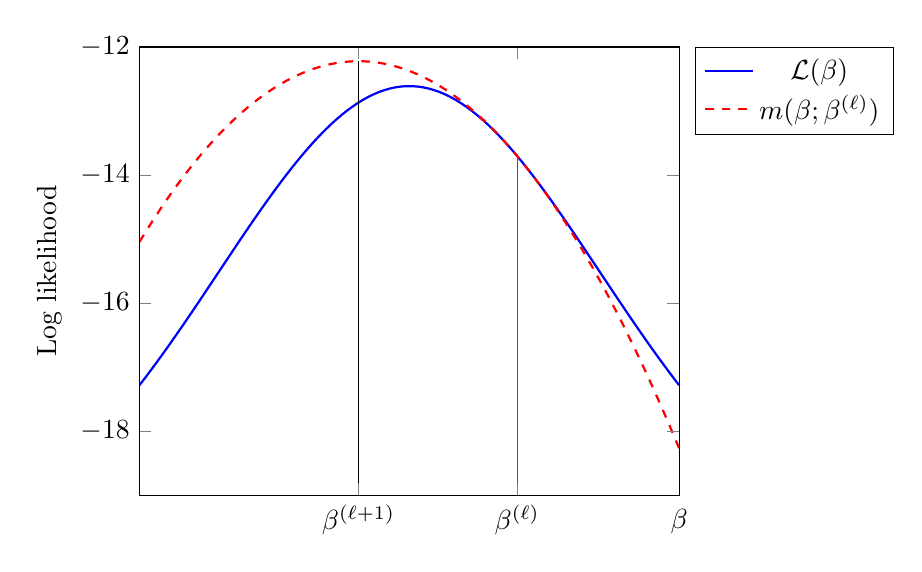
\begin{tikzpicture}[
  declare function = {
    f(\x) = exp(-\x * \x + 2) - 20 ;
    g(\x) = -2 * \x * exp(-\x*\x + 2) ;
    h(\x) = exp(-\x*\x + 2) * (4*\x*\x - 2) ;
    m(\x,\xk) = f(\xk) + (\x-\xk) * g(\xk) + 0.5 * (\x-\xk) * (\x-\xk) * h(\xk) ;
    xk = 0.4;
    fxk = f(xk) ;
    xkp1 = xk - g(xk) / h(xk) ;
    mxkp1 = m(xkp1, xk) ;
  }
 ]
  \begin{axis}[
      xlabel={$\beta$}, 
      xlabel style={at={(axis description cs:1, -0.01)}}, 
      ylabel={Log likelihood}, 
      samples=100, 
      domain=-1:1, 
      xmin=-1, 
      xmax=1, 
      ymin=-19, 
      ymax=-12, 
      axis on top, 
      xtick={xkp1, xk}, 
      xticklabels={$\beta^{(\ell+1)}$, $\beta^{(\ell)}$}, 
      legend pos=outer north east, 
    ]
  
    \addplot+[no marks, thick] {f(x)};
    \addlegendentry{$\mathcal{L}(\beta)$}
    \addplot+[no marks, thick, dashed] {m(x, 0.4)};
    \addlegendentry{$m(\beta;\beta^{(\ell)})$}
    \addplot +[mark=none] coordinates {
      (0.4, -19.0) (0.4, fxk)
    };
    \addplot +[mark=none] coordinates {
      (xkp1, -19.0) (xkp1, mxkp1)
    };
  \end{axis}
\end{tikzpicture}
